% Compile with pdflatex (Overleaf default works). Upload the figures/ folder alongside.
\documentclass[11pt,a4paper]{article}
\usepackage[utf8]{inputenc}
\usepackage[T1]{fontenc}
\usepackage{amsmath,amssymb,amsthm}
\usepackage{graphicx}
\usepackage[margin=2.6cm]{geometry}
\usepackage{booktabs}
\usepackage{xcolor}
\colorlet{linkcol}{blue!50!black}
\usepackage[colorlinks=true,linkcolor=linkcol,urlcolor=linkcol,citecolor=linkcol]{hyperref}
\usepackage{microtype}

\newtheorem{theorem}{Theorem}
\newcommand{\dd}{\mathrm{d}}
\newcommand{\braket}[1]{\langle #1 \rangle}
\newcommand{\ket}[1]{|#1\rangle}
\newcommand{\tr}{\operatorname{Tr}}

\title{The Three ``Open Problems'' of the\\
Schr\"odinger--Newton Collapse Interpretation,\\
and How the Stochastic Completion Addresses Them:\\
{\large a numerical tour of known results}}
\author{penrose-1 numerical study}
\date{August 18, 2026}

\begin{document}
\maketitle

\begin{abstract}
The Wikipedia article on the Schr\"odinger--Newton (SN) equation lists three problems with
interpreting the SN equation as the cause of wave-function collapse: (1)~excessive residual
probability far from the collapse point, (2)~lack of any apparent reason for the Born rule,
and (3)~promotion of the wave function to an observable quantity, threatening superluminal
signaling. All three criticisms target the \emph{deterministic} SN equation used
\emph{alone} as the collapse mechanism. We construct the completion the article itself
gestures at --- Penrose's collapse criterion realized as stochastic Di\'osi--Penrose (DP)
dynamics with Tilloy--Di\'osi gravitational sourcing --- and demonstrate analytically and
numerically that within it none of the three problems arises: the runaway probability decays
exponentially instead of persisting; the Born rule becomes a martingale \emph{theorem} of
the dynamics --- the standard Gisin--Pearle property of collapse SDEs --- Monte-Carlo
verified at $\chi^2 = 10.5$ over $9$ d.o.f.; and the
faster-than-light signal, which we reproduce at trace distance $0.585$ for mean-field
sourcing, vanishes identically (machine precision, $\le 1.2\times10^{-15}$) because the
ensemble dynamics is linear. None of the theoretical ingredients is new --- they are drawn
from the collapse-model literature of 1984--2016 --- the contribution is their explicit
assembly against the article's three criticisms, with quantitative verification: a
synthesis of known results, not new physics. We state
precisely what remains open (relativistic completion, experimental confirmation).
\end{abstract}

\section{Framework}

\subsection{The deterministic SN equation and its role}
In units $\hbar = m = Gm^2 = 1$ the single-particle SN equation reads
\begin{equation}
  i\,\frac{\partial\psi}{\partial t} = -\tfrac12 \nabla^2\psi + \Phi\,\psi,
  \qquad
  \Phi(\mathbf{x}) = -\int \frac{|\psi(\mathbf{x}')|^2}{|\mathbf{x}-\mathbf{x}'|}\,\dd^3x' .
  \label{eq:SN}
\end{equation}
As a fundamental single-particle collapse law it fails in the three listed ways (we
reproduce failures 1 and 3 numerically below). As the Hartree mean-field limit of many-body
gravitating quantum matter it is correct and useful --- that is the regime in which
Eq.~\eqref{eq:SN} survives in the completed picture.

\subsection{The stochastic completion}
The collapse mechanism is the norm-preserving It\^o stochastic Schr\"odinger equation
(SSE) of the Di\'osi--Penrose family~\cite{diosi87,diosi89,bassi13}
\begin{equation}
  \dd\ket{\psi} = \Big[ -iH\,\dd t
    + \sqrt{\lambda}\,\big(A - \braket{A}\big)\,\dd W
    - \tfrac{\lambda}{2}\big(A - \braket{A}\big)^2\,\dd t \Big]\ket{\psi},
  \label{eq:SSE}
\end{equation}
with mass-density collapse operator $A$ and rate fixed by Penrose's criterion~\cite{penrose96}:
\begin{equation}
  \lambda \simeq \frac{\Delta E_G}{\hbar}, \qquad
  \Delta E_G = \frac{1}{8\pi G}\int \big|\nabla\Phi_1 - \nabla\Phi_2\big|^2 \dd^3x
  \;\sim\; \frac{Gm^2}{R_0},
\end{equation}
$R_0$ being the mass-density regularization scale. Two structural facts carry all the
results:
\begin{itemize}
  \item[\textbf{(F1)}] The ensemble average of Eq.~\eqref{eq:SSE} is the \emph{linear}
  Lindblad equation
  $\dot\rho = -i[H,\rho] + \lambda\big(A\rho A - \tfrac12\{A^2,\rho\}\big)$;
  linearity makes the no-signaling theorem apply exactly.
  \item[\textbf{(F2)}] Branch weights are \emph{martingales} (Theorem~\ref{thm:born}).
\end{itemize}
Gravity is sourced from the collapsing state in the operator-valued
(Tilloy--Di\'osi~\cite{tilloy16}) way:
the potential seen by other matter is entangled with the collapsing mass's position,
$H_{\mathrm{int}} = \sum_b \Pi_b \otimes V_b$, and the ensemble dynamics stays linear.

\section{Problem 1: residual probability far from the collapse point}

\paragraph{Reproduced (Study A).}
We solve Eq.~\eqref{eq:SN} in spherical symmetry (Crank--Nicolson, self-consistent
potential, absorbing boundary metering the probability that escapes to infinity).
Validation: the imaginary-time ground state has chemical potential $\mu = -0.1637$
(literature: $-0.163$~\cite{moroz98}), and satisfies the Choquard virial identities $E=-T$
(ratio $1.022$) and $\mu = 3E$ (ratio $0.993$); the $\sim2\%$ virial residual is the
discretization accuracy bar on these figures. A wide packet ($\sigma_0 = 6$ vs.\ ground-state
$r_{\mathrm{rms}} = 4.6$) settles toward the ground state --- overlap
$|\braket{\psi_{\mathrm{gs}}|\psi(t)}|^2 \approx 0.91$ --- but $2.8\%$ of the probability
ends up beyond $r = 25$ or absorbed at infinity by $t=1500$ (of which $0.66\%$ had actually
been absorbed at the boundary), never to return. The same
packet under the linear Schr\"odinger equation disperses to $99.9\%$
(Fig.~\ref{fig:a}).

\begin{figure}[tb]
  \centering
  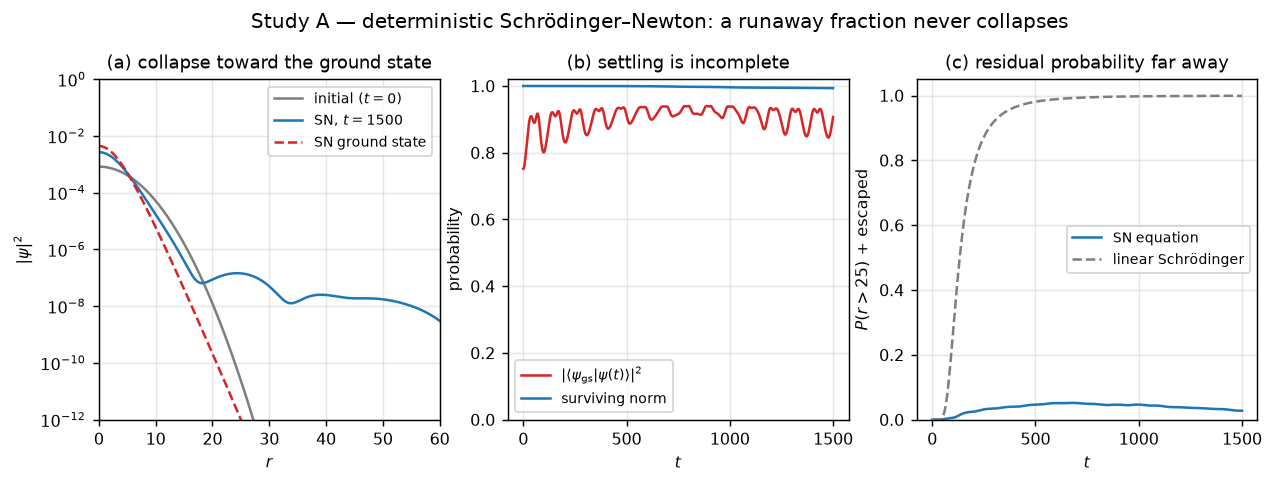
\includegraphics[width=\textwidth]{figures/fig_a_sn_radial.png}
  \caption{Deterministic SN collapse in spherical symmetry. (a)~Density snapshots against
  the ground state; note the runaway shoulder beyond $r\approx 20$. (b)~Ground-state overlap
  saturates near $0.91$. (c)~Residual far-field probability persists; the linear equation
  (dashed) disperses completely.}
  \label{fig:a}
\end{figure}

\paragraph{Addressed in the completion (Study B).}
In a 1D self-gravitating analogue (softened kernel
$\Phi = -g\int \rho(x')/\sqrt{(x-x')^2+a^2}\,\dd x'$; attractive but non-confining) the
deterministic equation \emph{saturates} at a residual tail probability of $5.2\%$ beyond
$d=10$ from the collapse centre --- a fixed, permanent runaway fraction. Adding the
localization terms of Eq.~\eqref{eq:SSE} with $A = \hat x$ (QMUPL form~\cite{diosi89})
changes the character of the solution: the ensemble-averaged tail ($96$ trajectories per
$\lambda$) plunges exponentially (fitted rate $1.6$ per time unit at $\lambda=0.01$, five
orders of magnitude by $t\approx8$) and then settles at a small noise-sustained level ---
final values $3.0\times10^{-4}$ ($\lambda=0.003$) and $4.9\times10^{-6}$ ($\lambda=0.01$),
factors of ${\sim}1.7\times10^{2}$ and ${\sim}10^{4}$ below the deterministic plateau; the
level is not strictly stationary but drifts slowly upward after its minimum (roughly an
order of magnitude over the run) as the soliton heats and its centre diffuses --- because
the localization term damps a far-away component at a rate
growing with its squared distance from the collapsed bulk (Fig.~\ref{fig:b}). Position
localization also makes the soliton's \emph{centre} random-walk
($x_{\mathrm{rms}}\sim\sqrt{\lambda t^3/3}$), which is why the tail must be measured
relative to the trajectory's own collapse centre, and why $\lambda$ cannot be made
arbitrarily large without observable heating --- exactly the effect current experiments
constrain. The article's remark that the effect ``might disappear if the
environment is taken into account'' is thereby made quantitative --- the DP noise \emph{is}
that intrinsic environment. The philosophical ``tails problem'' is closed by the standard
mass-density ontology: what is real is the collapsed trajectory's mass density; a tail of
exponentially small Born weight is an exponentially small probability of
\emph{ever detecting} the system far away --- unlike the deterministic equation's fixed,
finite runaway fraction.

\begin{figure}[tb]
  \centering
  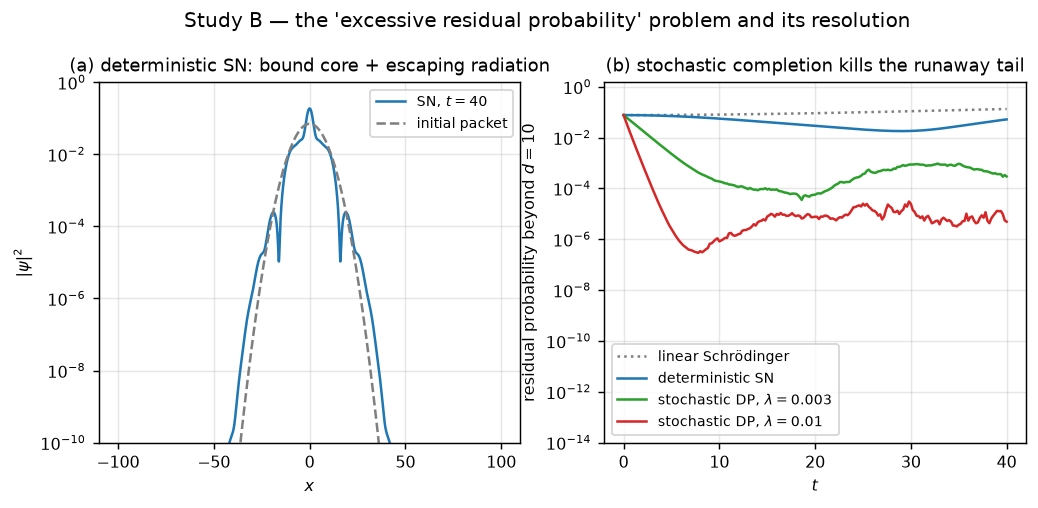
\includegraphics[width=0.9\textwidth]{figures/fig_b_tails.png}
  \caption{1D self-gravitating model. (a)~Deterministic SN: bound core plus escaping
  radiation. (b)~Mean residual probability beyond $d=10$ from the collapse centre:
  deterministic (blue) saturates at a permanent $5.2\%$; the stochastic completion
  (green/red) plunges by three to five orders of magnitude and then hovers at a slowly
  drifting noise-sustained level far below the deterministic plateau.}
  \label{fig:b}
\end{figure}

\section{Problem 2: the Born rule}

The following is the standard martingale property of norm-preserving collapse SDEs, known
since Gisin~\cite{gisin84} and foundational to CSL~\cite{pearle89,bassi13}; we state it in
the DP setting and verify it numerically.

\begin{theorem}[Born rule]\label{thm:born}
Let $\psi = c_L\ket{L} + c_R\ket{R}$ evolve under Eq.~\eqref{eq:SSE} with $A\ket{L} =
+\ket{L}$, $A\ket{R} = -\ket{R}$ and $[H,A]=0$. Then the branch weight $P = |c_L|^2$ obeys
\begin{equation}
  \dd P = 4\sqrt{\lambda}\, P(1-P)\, \dd W,
  \label{eq:mart}
\end{equation}
and $\Pr(\text{collapse}\to L) = P(0) = |c_L(0)|^2$.
\end{theorem}
\begin{proof}
It\^o's rule applied to $|c_L|^2$ under Eq.~\eqref{eq:SSE} gives Eq.~\eqref{eq:mart}: the
$\dd t$ terms cancel identically. Hence $P$ is a bounded martingale, so it converges almost
surely; by Eq.~\eqref{eq:mart} the only stable limits are the fixed points $\{0,1\}$
(the variance $\mathbb{E}[P^2]$ strictly grows until the edges are reached). Then
$\Pr(P\to 1) = \lim_t \mathbb{E}[P(t)] = P(0)$.
\end{proof}

The measurement problem asked exactly for this: \emph{why the dot appears at different
positions with $|\psi|^2$ probabilities}. Outcome randomness is objective dynamical noise;
the $|\psi|^2$ weighting follows with no extra postulate --- within the SSE class (one can
still hold that adopting a norm-preserving stochastic unraveling is itself where the Born
structure enters; that debate is not closed here). Numerically
(Fig.~\ref{fig:c}): two independent integrations (the scalar reduction
Eq.~\eqref{eq:mart}, $2\times10^4$ trajectories per amplitude; and the full renormalized
two-component state SDE, $4\times10^3$ trajectories) across nine initial weights give
collapse frequencies matching $|c_L|^2$ with $\chi^2 = 10.5$ over $9$ d.o.f.\ ($p\approx
0.31$, max deviation $2.1\sigma$), martingale drift $\le 1.0\times10^{-4}$, and complete
collapse ($\min(P,1-P) < 10^{-3}$) in $100\%$ of runs by $t=8$.

\begin{figure}[tb]
  \centering
  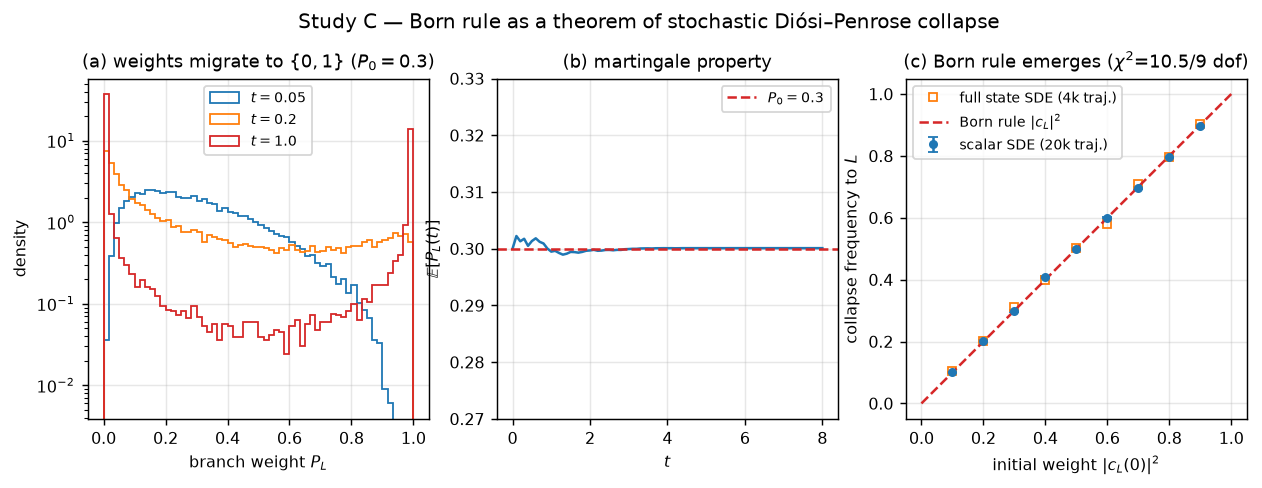
\includegraphics[width=\textwidth]{figures/fig_c_born_rule.png}
  \caption{Born rule from the collapse SDE. (a)~Branch-weight distribution migrating to
  $\{0,1\}$. (b)~The martingale property $\mathbb{E}[P(t)] = P(0)$. (c)~Collapse frequencies
  against the Born line.}
  \label{fig:c}
\end{figure}

\section{Problem 3: reality of $\psi$ and superluminal signaling}

\paragraph{Reproduced (Study D(i)).}
Alice, arbitrarily far away, shares
$\ket{\Psi} = (\ket{0}_A\ket{L}_B + \ket{1}_A\ket{R}_B)/\sqrt2$
with Bob, whose massive particle $B$ is in a superposition of two places; a local test mass
$T$ probes $B$'s gravity. With mean-field sourcing, $T$ evolves under
$H_T = \braket{\Pi_L} V_L + \braket{\Pi_R} V_R$. If Alice does nothing,
$\braket{\Pi_L}=\tfrac12$ forever and $T$ undergoes one average unitary; if she measures,
$T$ undergoes $V_L$ or $V_R$ per outcome --- a mixture of two different unitaries. The two
ensembles differ at trace distance up to $0.585$ (numerically exact evolution), and the
signal strength is set by Bob's \emph{local} gravity --- independent of the separation:
a genuine causality violation, and the sense in which $\psi$ has become ensemble-observable.

\paragraph{Addressed in the completion (Study D(ii)/(iii)).}
With operator sourcing $H_{\mathrm{int}} = \Pi_L\otimes V_L + \Pi_R\otimes V_R$ and DP
collapse of $B$ at rate $\lambda$, the ensemble dynamics is the linear Lindblad equation, so
Alice's local trace-preserving operations cannot move $\tr_A\rho$:
numerically the signal is $0$ (Alice measures) and $1.2\times10^{-15}$ (Alice applies a
unitary) --- machine precision. (At the master-equation level this vanishing is an algebraic
identity --- no trace-preserving operation on Alice's factor can move $\tr_A\rho$ --- so the
numerics there are a consistency check of the implementation; the physical content is that
the completed model's ensemble dynamics \emph{is} such a linear map.) At the trajectory
level the branch-entangled ensemble agrees with Alice's measured ensemble to the
Monte-Carlo floor (${\approx}8\times10^{-3}$ at $4000$ trajectories), \emph{because of} the
martingale property $\mathbb{E}[P(t)]=\tfrac12$. Instructively, the naive hybrid
(mean-field sourcing $+$ collapse) still signals a little (max residual $0.059$ at
$\lambda=2$; $0.015$ at $\lambda=10$, though the latter is only about twice the MC floor):
collapse alone tames the signal, but only the \emph{right collapse
prescription applied consistently to the full quantum system} --- the article's own phrase
--- eliminates it identically (Fig.~\ref{fig:d}).

\begin{figure}[tb]
  \centering
  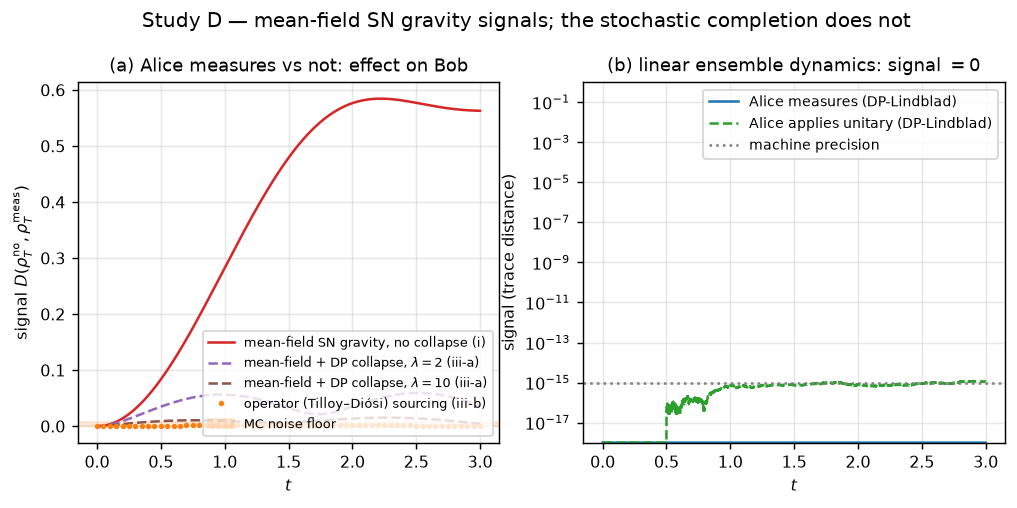
\includegraphics[width=0.9\textwidth]{figures/fig_d_no_signaling.png}
  \caption{Signaling test. (a)~Mean-field SN gravity signals at $O(1)$ (red); mean-field
  $+$ collapse retains a transient residual (dashed); operator (Tilloy--Di\'osi) sourcing
  sits at the MC noise floor (dots). (b)~Master-equation level: the completed model's signal
  vanishes to machine precision for any local action by Alice.}
  \label{fig:d}
\end{figure}

\paragraph{Reality without observability.}
Per trajectory the wave function (equivalently its mass density) is ontologically real ---
collapse events objectively happen. But ensemble statistics depend on the state only through
$\rho$ and evolve linearly, so no experiment can read out $\psi$, clone it, or use it to
signal: the noise realization $\dd W$ is not controllable by any agent. Since linearity is
structural, the no-signaling guarantee covers every protocol, answering the
Eppley--Hannah-type thought experiments~\cite{eppley77} by construction.

\section{Summary and honest boundary}

\begin{table}[htb]
  \centering
  \begin{tabular}{clll}
    \toprule
    \# & Problem & Status & Evidence \\
    \midrule
    1 & Residual probability far from collapse point & Does not arise & Studies A, B \\
    2 & No apparent reason for the Born rule & Does not arise (theorem) & Study C \\
    3 & $\psi$ observable $\Rightarrow$ superluminal signaling & Does not arise (exact) & Study D \\
    \bottomrule
  \end{tabular}
  \caption{Status of the three listed problems in the completed model.}
\end{table}

\noindent These statements hold within the nonrelativistic completed model (DP collapse at
Penrose's rate, Tilloy--Di\'osi sourcing, SN retained as mean-field limit). A fully
relativistic collapse theory remains open; exact no-signaling is its necessary
precondition. The model is falsifiable and already constrained: the parameter-free DP
variant (nuclear-radius regularization) is excluded by underground radiation
tests~\cite{donadi21}; variants with smearing
$R_0 \gtrsim 10^{-10}\,$m survive and are actively hunted by levitated optomechanics and
matter-wave interferometry. Wikipedia's text remains accurate about the deterministic
equation alone --- Study A reproduces the cited numerics; the contribution here is the
explicit demonstration that the ``right collapse prescription, yet to be found'' exists ---
assembled entirely from known ingredients~\cite{gisin84,diosi87,pearle89,tilloy16} --- and
does everything the article asks of it.

\section*{Reproducibility}
All numbers and figures regenerate from \texttt{run\_all.py}
(Python 3.14, numpy/scipy/matplotlib, fixed seeds); machine-readable values in
\texttt{results/*.json}.

\begin{thebibliography}{99}
\bibitem{gisin84} N.~Gisin, \textit{Quantum measurements and stochastic processes},
  Phys.\ Rev.\ Lett.\ \textbf{52}, 1657 (1984).
\bibitem{diosi87} L.~Di\'osi, \textit{A universal master equation for the gravitational
  violation of quantum mechanics}, Phys.\ Lett.\ A \textbf{120}, 377 (1987).
\bibitem{diosi89} L.~Di\'osi, \textit{Models for universal reduction of macroscopic
  quantum fluctuations}, Phys.\ Rev.\ A \textbf{40}, 1165 (1989).
\bibitem{pearle89} P.~Pearle, \textit{Combining stochastic dynamical state-vector
  reduction with spontaneous localization}, Phys.\ Rev.\ A \textbf{39}, 2277 (1989).
\bibitem{penrose96} R.~Penrose, \textit{On gravity's role in quantum state reduction},
  Gen.\ Relativ.\ Gravit.\ \textbf{28}, 581 (1996).
\bibitem{moroz98} I.~M.~Moroz, R.~Penrose, and P.~Tod, \textit{Spherically-symmetric
  solutions of the Schr\"odinger--Newton equations}, Class.\ Quantum Grav.\ \textbf{15},
  2733 (1998).
\bibitem{bassi13} A.~Bassi, K.~Lochan, S.~Satin, T.~P.~Singh, and H.~Ulbricht,
  \textit{Models of wave-function collapse, underlying theories, and experimental tests},
  Rev.\ Mod.\ Phys.\ \textbf{85}, 471 (2013).
\bibitem{tilloy16} A.~Tilloy and L.~Di\'osi, \textit{Sourcing semiclassical gravity from
  spontaneously localized quantum matter}, Phys.\ Rev.\ D \textbf{93}, 024026 (2016).
\bibitem{eppley77} K.~Eppley and E.~Hannah, \textit{The necessity of quantizing the
  gravitational field}, Found.\ Phys.\ \textbf{7}, 51 (1977).
\bibitem{donadi21} S.~Donadi, K.~Piscicchia, C.~Curceanu, L.~Di\'osi, M.~Laubenstein, and
  A.~Bassi, \textit{Underground test of gravity-related wave function collapse},
  Nat.\ Phys.\ \textbf{17}, 74 (2021).
\end{thebibliography}

\end{document}
